\title{Computer Networks - CS 214} % You may change the title if you want.

\author{Rishit Saiya - 180010027, Lab - 5 }

\date{\today}

\documentclass[12pt]{article}
\usepackage{fullpage}
\usepackage{enumitem}
\usepackage{amsmath,mathtools}
\usepackage{textcomp}
\usepackage{hyperref}
\usepackage{graphicx}
\begin{document}
\maketitle

The goal of this experiment was to emulate the TCP Congestion Control Algorithm where we dynamically varied the sender’s congestion window size as per the congestion control algorithm and then plot the change of CW with respect to number of updates made to CW.

It is to be noted that Go-back-N congestion control method has been used, but cumulative acknowledgments are not considered. For each segment, an individual timeout timer and ACK are used.

Throughout the emulation, the number of segments is set to be \textbf{40}.
The main parameters through which variation in CW size was varied were as follows:
\begin{itemize}
    \item Ki, the constant which alters the initial CW.
    \item Km, the multiplier constant of the CW during the exponential growth phase.
    \item Kn, the multiplier constant of the CW during the linear growth phase.
    \item Kf, the multiplier constant when the timeout occurs.
    \item Ps, the probability of receiving the ACK packet for a given segment before its timeout occurs.
\end{itemize}

The other variables that were involved emulating the Congestion Control Algorithm were as follows:
\begin{itemize}
    \item CW $\rightarrow$ Congestion Window Size, dynamically changing throughout the emulation.
    \item MSS $\rightarrow$ Maximum Segment Size is set to \textbf{1 KB/4 KB} depending upon user's choice.
    \item RWS $\rightarrow$ Receiver Window Size is set to \textbf{1 MB}.
    % \item Design and Analysis of Algorithms
    \item N $\rightarrow$ A parameter defined whose value is $\lceil \frac{CW}{MSS} \rceil$.
\end{itemize}

In the equations, the notation is as per the programming logic. [Same variable on either side of the equation denotes that the variable appearing in the RHS takes its old value and is dynamically changes in the program.]

The ssthresh is the Threshold Limit which is threshold limit considered during the complete emulation of Congestion Control Algorithm. ssthresh is set to \textbf{2 KB}.

\textbf{\textit{All the equations used in this report are in correspondence with the research papers provided and are completely proved and verified.}}

%--------------------------END PROLOGUE---------------------------------

\section{Variation of Congestion Window Size with Ki}
As it is evident from above mentioned points that, Ki is triggering the changes in the initial congestion window.
The variation in Ki was done with other parameters set as follows:
\begin{itemize}
    \item Km = 2
    \item Kn = 0.5
    \item Kf = 0.5
    \item Ps = 0.03
    
\end{itemize}

The iterating values for Ki were:
\begin{itemize}
    \item Ki value for generation of ki\_1.txt was 1.
    \item Ki value for generation of ki\_2.txt was 2.
    \item Ki value for generation of ki\_3.txt was 3.
    \item Ki value for generation of ki\_4.txt was 4.
\end{itemize}

\begin{figure}
    \centering
    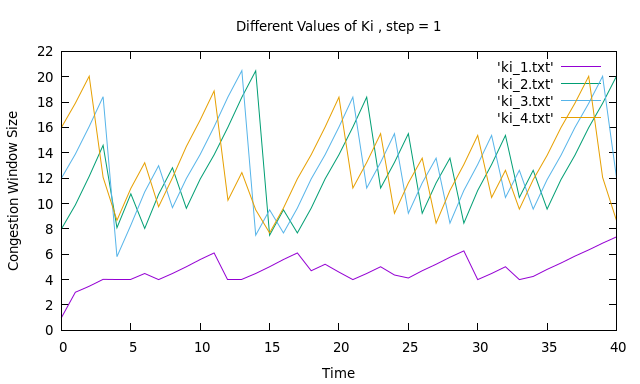
\includegraphics[width=15cm, height=10cm]{ki.png}
    \caption{Variation of CW with varying Ki}
    % \label{My figure}
\end{figure}

From Figure 1, it is evident that $CW_{initial}$ is increasing with increasing values of Ki.

This further is substantiated by the equation:
\begin{equation*}
    CW = Ki \times MSS
\end{equation*}

Since Ki is increasing and CW is directly proportional to Ki whilst MSS being constant, CW also increases.
%------------------------------END OF Ki------------------------------

\section{Variation of Congestion Window Size with Km}
As it is evident from above mentioned points that, Km is the multiplier that is changing initial Congestion Window in the exponential growth phase.
The variation in Ki was done with other parameters set as follows:
\begin{itemize}
    \item Ki = 1
    \item Kn = 0.5
    \item Kf = 0.5
    \item Ps = 0.03
\end{itemize}

The iterating values for Km were:
\begin{itemize}
    \item Km value for generation of km\_1.txt was 0.5.
    \item Km value for generation of km\_2.txt was 1.
    \item Km value for generation of km\_3.txt was 1.5.
    \item Km value for generation of km\_4.txt was 2.
\end{itemize}

\begin{figure}
    \centering
    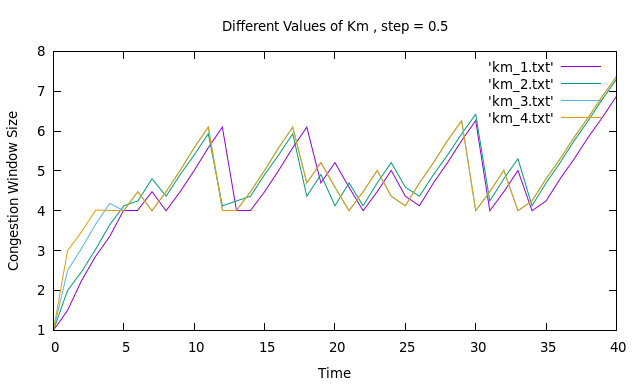
\includegraphics[width=15cm, height=10cm]{km.png}
    \caption{Variation of CW with varying Km}
    % \label{My figure}
\end{figure}

From Figure 2, it is evident that CW is exponentially increasing and nearly converged to same values of CW for different values of Km. Furthermore, the whole variation of CW over different values of Km nearly resulted in same curves of CW vs. Time.

This is governed by the equation:
\begin{equation*}
    CW = min(CW + Km \times MSS, RWS)
\end{equation*}

Since the CW is governed by Km and old CW and clearly Km is positive and greater than 1, so in the exponential phase it is increasing. Further more we see its range is in between 4 and 7 only. This is due to RWS factor in the above equation. It saturates further increase and if the congestion occurs there, it is by equations that ssthresh will become half of CW and CW will be set there.

%------------------------------END OF Km------------------------------

\section{Variation of Congestion Window Size with Kn}
As it is evident from above mentioned points that, Kn is the multiplier that is changing initial Congestion Window in the linear growth phase.

The variation in Ki was done with other parameters set as follows:
\begin{itemize}
    \item Ki = 1
    \item Km = 2
    \item Kf = 0.5
    \item Ps = 0.03
\end{itemize}

The iterating values for Km were:
\begin{itemize}
    \item Kn value for generation of kn\_1.txt was 0.5.
    \item Kn value for generation of kn\_2.txt was 1.
    \item Kn value for generation of kn\_3.txt was 1.5.
    \item Kn value for generation of kn\_4.txt was 2.
\end{itemize}

\begin{figure}
    \centering
    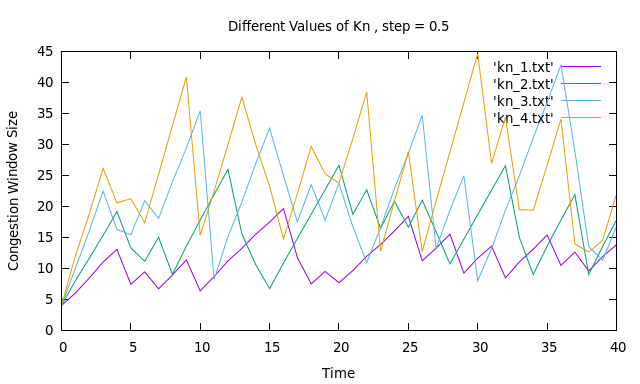
\includegraphics[width=15cm, height=10cm]{kn.png}
    \caption{Variation of CW with varying Kn}
    % \label{My figure}
\end{figure}

From Figure 3, it is evident that CW is exponentially increasing and nearly converged to same values of CW for different values of Km.
But the variation over the time is very non uniform. 

This is governed by the equation:
\begin{equation*}
    CW = min(CW + Kn \times MSS \times \frac{MSS}{CW}, RWS)
\end{equation*}

This is due to involvement of other variables such as CW and MSS. Due to dynamically changing value of CW, the non-uniform are generated. However at the end we see that all the curves nearly converge to the same values of CW.

%------------------------------END OF Kn------------------------------

\section{Variation of Congestion Window Size with Kn}
As it is evident from above mentioned points that, Kf is the constant that triggers the changes in the Congestion Window when congestion occurs.

The variation in Kf was done with other parameters set as follows:
\begin{itemize}
    \item Ki = 1
    \item Km = 2
    \item Kn = 0.5
    \item Ps = 0.03
\end{itemize}

The iterating values for Kf were:
\begin{itemize}
    \item Kf value for generation of kf\_1.txt was 0.1.
    \item Kf value for generation of kf\_2.txt was 0.2.
    \item Kf value for generation of kf\_3.txt was 0.3.
    \item Kf value for generation of kf\_4.txt was 0.5.
\end{itemize}

\begin{figure}
    \centering
    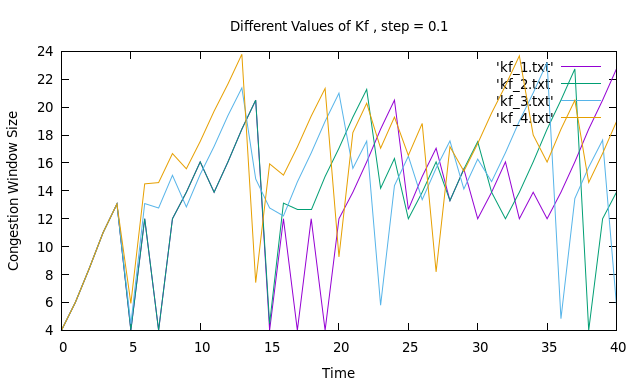
\includegraphics[width=15cm, height=10cm]{kf.png}
    \caption{Variation of CW with varying Kf}
    % \label{My figure}
\end{figure}

From Figure 4, it is evident that CW is uniformly increasing till the $1^{st}$ congestion has occurred. After that the variation is very random.

This is governed by the equation:
\begin{equation*}
    CW = max(1, Kf \times CW)
\end{equation*}

As it depends on Kf passed in CLI and also the random number generated between 0 and 1 to compare it with Ps. Basically, there is a contribution of $rand()$ in the decision whether the congestion is going to occur or not.

%------------------------------END OF Kf------------------------------

\section{Variation of Congestion Window Size with Ps}
As it is evident from above mentioned points that, Ps is the probability of receiving the ACK packet for a given segment before its timeout occurs.

The variation in Ps was done with other parameters set as follows:
\begin{itemize}
    \item Ki = 1
    \item Km = 2
    \item Kn = 0.5
    \item Kf = 0.5
\end{itemize}

The iterating values for Ps were:
\begin{itemize}
    \item Ps value for generation of ps\_1.txt was 0.1.
    \item Ps value for generation of ps\_2.txt was 0.2.
    \item Ps value for generation of ps\_3.txt was 0.3.
    \item Ps value for generation of ps\_4.txt was 0.4.
\end{itemize}

\begin{figure}
    \centering
    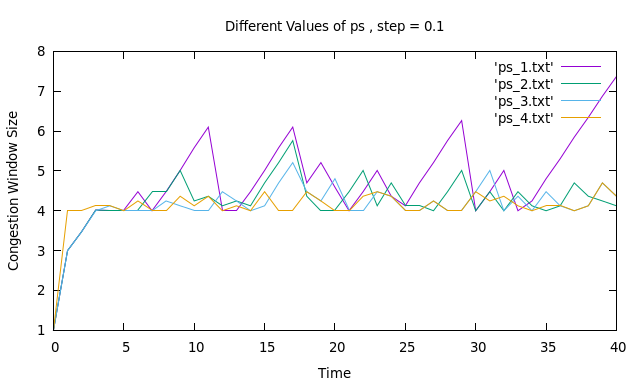
\includegraphics[width=15cm, height=10cm]{ps.png}
    \caption{Variation of CW with varying Ps}
    % \label{My figure}
\end{figure}

From Figure 5, it is evident that CW is varying non-uniformly.

This is governed by the equation:
\begin{equation*}
    Ps \in [0,1]
\end{equation*}

% There will always be some point of congestion irrespective of Ps and hence all the graphs remains the same.
We can see that greater the value of Ps, greater are the chances of congestion.

If the r \textless \, Ps, then Congestion occurs, where r is the random number generated by rand() function and r $\in$ [0,1].
%------------------------------END OF Ps------------------------------
\end{document}